\documentclass[DM,lsstdraft,toc,usenatbib]{lsstdoc}

% Package imports go here
\usepackage{amsmath}	% Advanced maths commands
\usepackage{amssymb}
\usepackage{gensymb}  % degree symbol 
\usepackage{natbib}  % bibliography
\usepackage{cprotect} 
% Local commands go here

%% Journal abbreviations
%\bibliographystyle{aasjournal}

\title[Crowded fields ]{LSST  Crowded Fields photometry}

\author{
K.~Suberlak, C.~Slater,
\v{Z}.~Ivezi\'c, P.~Yoachim}

\setDocRef{LSST-2017}
\date{\today}
\setDocRevision{TBD}
\setDocStatus{draft}
\setDocAbstract{%
A report on the performance of current LSST Stack pipelines in crowded stellar fields. Using the real data we explore the metrics that could be used to direct decision-making process for pipeline improvements. The quality metrics show also a way to validate the performance of LSST pipelines  after major software upgrades.}

% Change history defined here. Will be inserted into
% correct place with \maketitle
% OLDEST FIRST: VERSION, DATE, DESCRIPTION, OWNER NAME
\setDocChangeRecord{%
\addtohist{1}{2017-07-16}{First draft.}{Krzysztof Suberlak}
\addtohist{2}{2017-10-19}{Updated outline.}{Krzysztof Suberlak}
\addtohist{2}{2018-01-25}{Major revision.}{Krzysztof Suberlak}
}

\begin{document}

% Create the title page
% Table of contents will be added automatically if "toc" class option
% is used.
\maketitle

\section{Introduction}

We report on the performance of the Large Scale Synoptic Telescope (LSST) science pipelines \footnote{\url{https://pipelines.lsst.io}}, also known as 'the LSST stack', in stellar fields of varying levels of crowdedness.

The LSST will sample every night over 1,000  regions in the sky , delivering terabytes of raw data in need of processing: photometric  and astrometric calibration, to deliver a calibrated exposure image, as well as a source catalog, among other image products\footnote{\url{http://ls.st/LSE-163}}~\cite{narayan2018}.

The survey sky is composed of regions very diverse in terms of stellar density, or crowdedness:  from high density low-galactic latitude regions that have tens of millions of sources per square degree, to low-density regions towards the galactic poles with less than thousand sources per square degree. 

Deblending and successful photometry is an inherent part of any astronomical data processing pipeline.  There exists a body of research answering questions that are specific to crowded stellar fields, eg. how many beams do we need per source (see ~\citep{hogg2001}), or how  the crowded fields photometry can be approached in the era of large telescopes ~\cite{olsen2003} Other studies involved eg. HyperSuprime CAM pipeline ( developed in parallel with the LSST Stack), recognizing that the deeper the survey, the higher the stellar densities encountered, and the onset of blurring the the boundaries between deblending, measurement, and detection~\cite{bosch2017}. 

In this report we compare the 'out-of-the-box' LSST Stack tools, in particular processCcd.py, to the DECAm [Galactic] Plane Survey (DECAPS) catalogs based on the NOAO state-of-the-art community pipeline (~\cite{schlafly2017}). First we use the LSST Metrics Analysis Framework Galfast simulation of the night sky find regions representing various stellar densities - see Sec.~\ref{sec:MAF}. Then we query the DECAPS image database for images that were taken at exposures and filters that reach similar depth to the LSST single-visit depth (Sec.~\ref{sec:DECAPS}). We select few DECAPS exposures at each density level, and process with LSST Stack tools (Sec.~\ref{sec:LSST}). In Sec.~\ref{sec:metrics} we compare the results of LSST processing and the DECAPS single-epoch catalogs, and develop the quality metrics.  Finally in Sec.~\ref{sec:conclusions} we make recommendations for future work. 


\section{Identifying density regions}
\label{sec:MAF}
To identify regions representing different stellar densities we use the LSST  Metrics Analysis Framework \footnote{\url{https://www.lsst.org/scientists/simulations/maf}, and \url{https://github.com/lsst/sims_maf}} simulated stellar density map prepared by P. Yoachim and L. Jones 
\footnote{\url{sims_maf/python/lsst/sims/maf/maps/createStarDensitymap.py}}
%\url{https://github.com/lsst/sims_maf/blob/a9bc8f6d00fae5d7ce4ff6ea7279d5a0fca29437/python/lsst/sims/maf/maps/createStarDensitymap.py}}. 

The  resulting dataset \verb|starDensity_r_nside_64.npz| contains 64 magnitude bins, with the entire sky divided into 49152  healpixels \footnote{\url{http://healpix.sourceforge.net}}. Each healpixel contains information about the number of stars per square degree in a given magnitude bin in the simulated sky - see Fig.~\ref{fig:MAF_densities}.

\begin{figure}
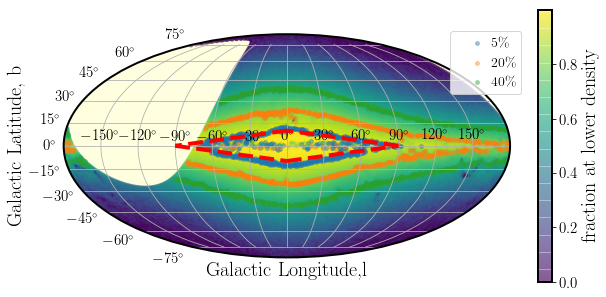
\includegraphics[width=1.0\columnwidth]{figs/MAF_densities.png}
%\vskip -0.15in
\caption{MAF healpixels plotted in galactic coordinates in Mollweide projection. The brightest regions correspond to highest stellar densities. The missing part in the higher declination is the part of the sky above $\delta>40 \degree$, which is not observable from the southern location of Cerro Pach\'on.}
\label{fig:MAF_densities}
\end{figure} 


To match the LSST single-visit depth,  we select magnitude bins smaller than r=24.5.   For each healpixel we calculate the number of pixels that have a higher stellar count.  Since each healpixel has an equal area, the fraction of pixel number above a certain threshold corresponds to the fraction of sky area above given density limit.  Fig.~\ref{fig:illustrate_density} illustrates how we define percentiles of stellar densities, so that eg. 'top 1\%' density means that only 1 in 100 pixels has a higher density than a given pixel, and 'top 10\%' means that '10 \%' of pixels in the considered simulation of the sky. 

\begin{figure}
\includegraphics[width=0.7\columnwidth]{figs/All_sky_r_lt245_twiny.png}
%\vskip -0.15in
\caption{We order all healpixels in the MAF simulation of LSST sky in terms of stellar count per pixel. For each healpixel we calculate the number of pixels at greater or equal stellar count, which corresponds to the area of the sky at greater density.  Normalizing that by the total number of pixels we obtain a fraction of the sky at greater or equal density, similar to the cumulative distribution. Horizontal dashed lines illustrate selecting pixels at 5\% or 10\% density. }
\label{fig:illustrate_density}
\end{figure} 


Since this definition of density includes all pixels that are within 'top 20\%', we take selection around the percentiles so that :

\begin{itemize}
\item top  1 \%  means  fraction of sky with greater density is 0.01
\item 5 \% region means such that between  4\% and 6\%
\item 20 \% region  includes   19\% - 21\%
\item 50 \% region includes 49\% - 51\% 
\end{itemize}


We illustrate the location of pixels representative of these density brackets on the sky in Fig.~\ref{fig:mollw_galactic}. 


\begin{figure}
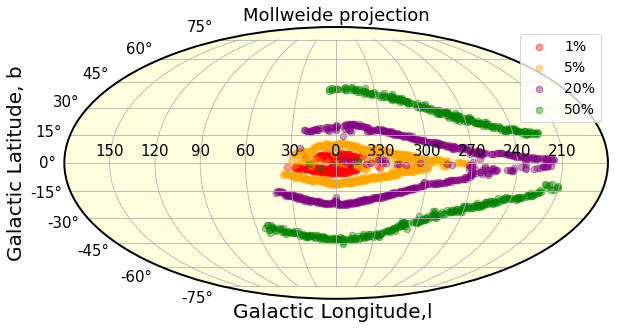
\includegraphics[width=1.0\columnwidth]{figs/Illustrate_density_regions_mollw_galactic.png}
%\vskip -0.15in
\caption{Illustration of location of regions representative of different relative density in cylindrical projection, galactic coordinates. The highest density regions are located close to the galactic bulge, and the decreasing density regions approximately trace isophotes of the Milky Way. The 20\% regions close to the galactic equator correspond to high extinction regions that appear to have less counts due to interstellar dust. }
\label{fig:mollw_galactic}
\end{figure} 


\section{DECam Plane Survey }
\label{sec:DECAPS}
To analyze the performance of the LSST Stack with real data, we used the Dark Energy Camera (DECam) imaging, taken as part of the  DECam Plane Survey (DECAPS)~\cite{schlafly2017}, at the 4-m Cerro Tololo Inter-American Observatory telescope (CTIO)\footnote{see \url{http://www.ctio.noao.edu/noao/node/1033}}. On Fig.~\ref{fig:decaps_fields} we overlay the locations of all DECAPS fields on top  the MAF map of the LSST sky. All DECAPS single-epoch images were processed with the DECAPS pipeline, resulting in single-epoch catalogs.  The headers of all catalogs were assembled into the image database that contains information about single-visit exposure time, filter,  time of observation, position, etc.  It was used to select DECAPS fields with single-epoch depth similar to that of the single-visit depth of 30 sec LSST exposure. Thus we selected DECAPS fields with  exposure between 90  and 125 sec, taken in   u, g, r,  or VR filter. 

\begin{figure}
\includegraphics[width=1.0\columnwidth]{figs/MAF_DECAPS_sources.png}
%\vskip -0.15in
\caption{All DECAPS fields, overlaid on the map of healpixel stellar densities from MAF simulated sky.  We matched the position of the center of each DECAPS field to the nearest healpixel to obtain an estimate of stellar density at each DECAPS field. In this way we selected DECAPS fields representative of various stellar densities (eg. 5\%, 10\%, 15\%, as explained in Sec.~\ref{sec:MAF}). }
\label{fig:decaps_fields}
\end{figure} 


We cross-matched the DECAPS image database with the  stellar density information contained in MAF healpixels. Each DECAPS image plane is tiled by a mosaic of 62 CCDs (see Fig.~\ref{fig:decam_mosaic_ccd}). The size of each CCD element of the DECAm image plane mosaic is 2046x4094 pixels, with pixel scale of 0.27 arcsec / px , so that a single mosaic element covers an area of 0.047117 square \degree. A single DECam exposure is also called a visit, and with 62 mosaic elements the full field of view  2.2\degree wide is several times bigger than the full moon. This makes it comparable to the LSST 3.5\degree wide field of view.  Using the coordinates of the center of each DECAPS field  we found the nearest healpixel within 0.5\degree . 
% Matching MAF healpixels are at locations very close to that of the DECam images, since if we consider the full DECam image mosaic being inscribed in a rectangle, it would  have a diagonal of approximately 1.5\degree, or a circle that has a  radius of approximately 0.75\degree. 

\begin{figure}
\includegraphics[width=1.0\columnwidth]{figs/Fig_4-3_NOAO_DECam_ccd_mosaic.png}
%\vskip -0.15in
\caption{An illustration of the DECam CCD mosaic image plane, adapted from Fig.4-3 in NOAO Data Handbook ~\citep{shaw2015}, . The color corresponds to the one of the four sets of read-out electronics (orange,pink, blue,yellow), or the guiding (green) and focus (magenta) CCDS.  The grey CCDs do not function properly. For this reason  S30, S7, and N30 were excluded from the analysis. }
\label{fig:decam_mosaic_ccd}
\end{figure} 


\section{LSST Processing of DECAPS data}
The DECAPS calibrated imaging was processed with the LSST Science Pipelines installed on the LSST-dev machine installed at the NCSA.  We specifically employed processCcd.py and the standard Stack configuration. Transferring the resulting source catalogs and calexp files over scp we analyzed the output on a laptop with jupyter notebooks. 


To obtain independent order of magnitude comparison to MAF simulation, and LSST/DECAPS processing of DECam data, we also queried TRILEGAL simulation data, and processed the DECam images  with DAOPhot - see Appendix~\ref{sec:appendixA}. 

The big picture is to find how metrics that we develop behave as a function of source crowdedness. We consider completeness, and photometric accuracy. 

\subsection{Cleaning DECAPS catalog, comparison to LSST pixel mask}
To compare LSST and DECAPS catalogs, we cleaned both catalogs with the flags assigned to each source by the respective image processing pipeline. To verify the validity of DECAPS source flags, we compared them with the LSST pixel-level mask information stored in the FITS Header Data Unit. Pixel-level masks are encoded in 8 bits,  each of which can be 'on' or 'off', signifying that a given flag was 'on' or 'off' for a given pixel. The total value of the mask at each pixel is a decimal representation of such eight bits binary number, eg.  $(00100001)_{2} = 2^{0} + 2^{5}  = 1 + 32 = (33)_{10} $ means that bit $'0'$ and $'5'$ are 'on' (counting from the right). See Table~\ref{tab:lsst_flags} for details. 


\begin{table}
\centering
\caption{LSST pixel mask bit values.}
\label{tab:lsst_flags}
\begin{tabular}{ ccc} 
\hline
Bit position & Description & Mask decimal value  \\ 
\hline
0  & bad               & 1    \\ 
1  & saturated         & 2   \\ 
2  & interpolated      & 4    \\ 
3  & cosmic ray        & 8    \\ 
4  & edge              & 16    \\ 
5  & detected          & 32   \\ 
6  & detected negative & 64   \\ 
7  & suspect           & 128   \\ 
8  & no data           & 256     \\ 
\hline
\end{tabular}
\end{table}

For each  visit we considered DECAPS single-epoch source catalog, and the LSST calexp image.  For each DECAPS source, given the pixel coordinates, we retrieved the value of the LSST mask at that pixel. Given the understanding of the LSST flag bits (Table~\ref{tab:lsst_flags})  we performed a bitwise and with a mask filter$(11011111)_{2} = (2^{1}+2^{2}+2^{3}+2^{4}+2^{6}+2^{7})_{10}$, flagging a source as 'lsst bad' if either of the flag bits apart from '5' (detected) was 'on'. 
Each DECAPS source  also has a flag where the value is composed of bits inherited from the NOAO Community Pipeline (see Table~\ref{tab:decaps_flags}). We performed a bitwise and with the mask filter $(2^{1}+ 2^{3}+  2^{4}+  2^{5}+  2^{6}+  2^{8}+  2^{20}+  2^{22})_{10}$, flagging the source as 'decaps bad' if either of this bits were 'on'. We compared which sources would be excluded based on the DECAPS source-level flags vs LSST pixel-level masks, and we found that for a particular visit 611980 the overlap between sources excluded based on LSST pixel mask vs DECAPS source flags is 99\%. This means that DECAPS flagging is consistent with the LSST mask information, and the same sources would be 'excluded' based on either DECAPS flags or LSST mask information. 
For this reason we cleaned the DECAPS catalog with  source level flags. 
 
\subsection{Cleaning LSST catalog}
The LSST source catalog contains per source a list of 83 flags that could be set 'on' or 'off'. Of these, flags number 60:72 are \verb|base_PixelFlags_flag|, meaning they contain information relevant to the level of source detection, rather than processing. See Table~\ref{tab:lsst_src_flags} for detailed descrition. 

\begin{table}
\centering
\caption{LSST source explanation. All flags names start with 'base\_PixelFlags\_flag\_' which was omitted in the flag\_name column below. }
\label{tab:lsst_src_flags}
\begin{tabular}{ccc}
\hline
number & name & explanation \\
\hline
60 & flag & general failure flag, set if anything went wrong \\
61 & offimage & Source center is off image \\
62 & edge & Source is outside usable exposure region (masked EDGE or NO\_DATA) \\
63 & interpolated & Interpolated pixel in the Source footprint \\
64 & saturated & Saturated pixel in the Source footprint \\
65 & cr & Cosmic ray in the Source footprint \\
66 & bad & Bad pixel in the Source footprint \\
67 & suspect & Source's footprint includes suspect pixels \\
68 & interpolatedCenter & Interpolated pixel in the Source center \\
69 & saturatedCenter & Saturated pixel in the Source center \\
70 & crCenter & Cosmic ray in the Source center \\
71 & suspectCenter & Source's center is close to suspect pixels \\
72 & flag & General Failure Flag \\
\hline
\end{tabular}
\end{table}

We clean the LSST source catalog from sources that have flags number 62 (edge) or 67 (interpolatedCenter). Other flags would remove too many sources that have only small 'defects', eg. 64 (interpolated) is on for a bright source on the footprint of which there is a cosmic ray, and 65 (bad) is on for any source which has even one bad pixel in the footprint -see Fig.~\ref{fig:lsst_src_flags}


\begin{figure}
\includegraphics[width=1.0\columnwidth]{figs/LSST_mask_611980ccd01_61_67.png}
%\vskip -0.15in
\caption{Sources from LSST source catalog for CCD 01 , visit 611980,  for which flags 61 or 67 were 'on'. This cleans sources that were either on the CCD edge, or have been interpolated at the center. This properly removes the cosmic rays and edges, while preserving other sources that may have eg. a single bad pixel , or cosmic ray going across the footprint. }
\label{fig:lsst_src_flags}
\end{figure} 



\subsection{Completeness}
For each visit, that corresponds to a given level of crowdedness, we consider the completeness of the LSST source catalog to the DECAPS single-epoch source catalog. From both catalogs apart from performing cleaning based on flag information we removed sources with signal-to-noise ratio smaller than five:  $S/N < 5$. These catalogs were positionally cross-matched, with the peak of separation at less than 0.3 arcseconds (see Fig.~\ref{fig:separation_histogram})  


\begin{figure}
\includegraphics[width=1.0\columnwidth]{figs/decaps_lsst_separation_NEW.png}
%\vskip -0.15in
\caption{The histogram of separation of cross-matched sources between LSST and DECAPS catalogs for visits at various source densities (g1,g2 correspond to different locations of observations in g filter at the same density level). Choosing to consider a 'match' sources that are within 0.5 arcsec separation is well justified given this plot. }
\label{fig:separation_histogram}
\end{figure} 


We consider two sources from LSST vs DECAPS catalogs a match if they are within 0.5 arcseconds (Fig.~\ref{fig:separation_histogram}) and 0.5 magnitude difference (Fig.~\ref{fig:dmag_scatter}) . Thus in a given magnitude bin, completeness is defined by the percentage of DECAPS sources that have an LSST match (see Fig.~\ref{fig:completeness}). 




\begin{figure}
\begin{centering}
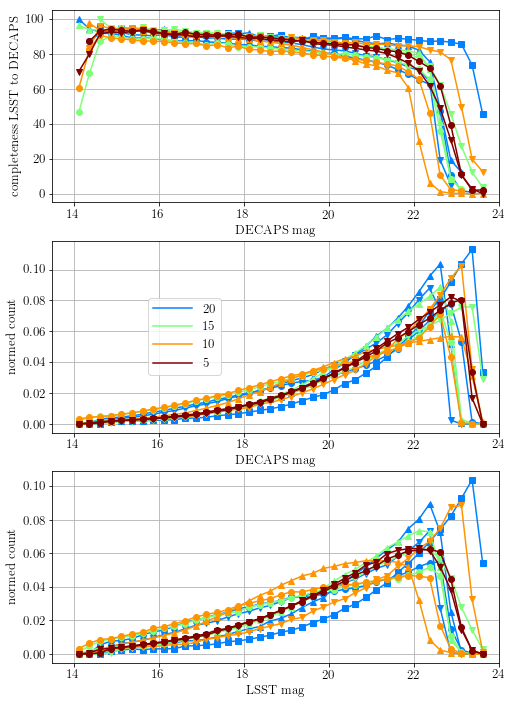
\includegraphics[width=0.7\columnwidth]{figs/completeness_count_lsst_decaps.png}
%\vskip -0.15in
\caption{Different colors correspond to different level of stellar crowdedness (5 is more dense,  20 is least dense, as defined earlier). The top panel depicts the completeness of DECAPS sources to LSST binned along DECAPS magnitudes. The middle panel the count of cleaned DECAPS catalog, and the bottom panel the count of cleaned LSST catalog, before they are cross-matched. Despite different densities, there is not much variation in the level of completeness , which may vary even for different fields at similar source densities (distinguished by different markers).}
\label{fig:completeness}
\end{centering}
\end{figure} 

We illustrate the DECAPS-LSST 'matches' and 'mismatches' for visit 611980 CCD01 on Figs.~\ref{fig:matches_ill_d2d},~\ref{fig:matches_ill_d2d_mask}, and CCD10 on Figs.~\ref{fig:ccd10_d2d_mask},~\ref{fig:ccd10_d2d_all} and ~\ref{fig:ccd10_d2d_plain}


% VISIT 611980  ,  HORIZONTAL BAD PIXELS .... 
\begin{figure}
\begin{centering}
\includegraphics[width=0.7\columnwidth]{figs/visit_611980_ccd0110-24d2d_all.png}
%\vskip -0.15in
\caption{We consider cleaned DECAPS and LSST catalogs. All LSST sources are marked in green, and all DECAPS sources with an LSST counterpart are marked in magenta. The DECAPS sources missing LSST counterpart within 0.5 '' are shown in red. }
\label{fig:matches_ill_d2d}
\end{centering}
\end{figure} 

\begin{figure}
\begin{centering}
\includegraphics[width=0.7\columnwidth]{figs/visit_611980_ccd0110-24d2d_mask.png}
%\vskip -0.15in
\caption{The same as Fig.~\ref{fig:matches_ill_d2d}, but showing the LSST pixels that have bits  0,1,2,3,4,6,7,8 'on' in dark shading (see Tab.~\ref{tab:lsst_flags}). In particular, the horizontal stripes on the bottom correspond to bit 0 ('bad').}
\label{fig:matches_ill_d2d_mask}
\end{centering}
\end{figure} 


% Visit 611980 , CCD 10 :  GALAXY SHREDDING 
\begin{figure}
\begin{centering}
\includegraphics[width=0.7\columnwidth]{figs/visit_611980_ccd1010-24d2d_mask.png}
%\vskip -0.15in
\caption{Like on Fig.~\ref{fig:matches_ill_d2d_mask} we overlay the LSST pixel mask data on top DECAPS sources that do (magenta) and do not  (red) have an LSST counterpart within 0.5 ''. }
\label{fig:ccd10_d2d_mask}
\end{centering}
\end{figure} 


\begin{figure}
\begin{centering}
\includegraphics[width=0.7\columnwidth]{figs/visit_611980_ccd1010-24d2d_all.png}
%\vskip -0.15in
\caption{The same region of visit 611980, CCD10, as Fig.~\ref{ccd10_d2d_mask}, showing all LSST sources, as well as DECAPS sources that do (magenta), and do not (red) have an LSST match. }
\label{fig:ccd10_d2d_all}
\end{centering}
\end{figure} 


\begin{figure}
\begin{centering}
\includegraphics[width=0.7\columnwidth]{figs/visit_611980_ccd1010-24d2d_good.png}
%\vskip -0.15in
\caption{Compare to Fig.~\ref{fig:ccd10_d2d_all} - here we marked only the DECAPS sources that have an LSST match within 0.5 '', and all LSST sources, removing the red DECAPS sources that did not have an LSST match. This allows to notice the galaxy in the lower left corner that was shredded by DECAPS pipeline to point sources.  }
\label{fig:ccd10_d2d_plain}
\end{centering}
\end{figure} 


\subsection{Photometric accuracy}

\begin{figure}
\begin{centering}
\includegraphics[width=0.6\columnwidth]{figs/decaps_lsst_dmag_density_15.png}
%\vskip -0.15in
\caption{Difference in magnitudes between the DECAPS and LSST magnitudes for sources matched within 0.5 arcsec for a region in top 15\% density (611970) . While in calculating completeness apart from spatial proximity we require sources to be within 0.5 mag to constitute a 'match', here we did not exclude any outliers in calculating the median and $\sigma_{G}$, since these statistics are insensitive to outliers.  We overplot the median with yellow circles, and the $\pm \sigma_{G}$ envelope - the measure of scatter based on the interquartile range. The offset between LSST and DECAPS is on the level of 0.05 mag. The same quantities plotted for all fields can be shown on Fig.~\ref{fig:dmag_spread} }
\label{fig:dmag_scatter}
\end{centering}
\end{figure} 

\begin{figure}
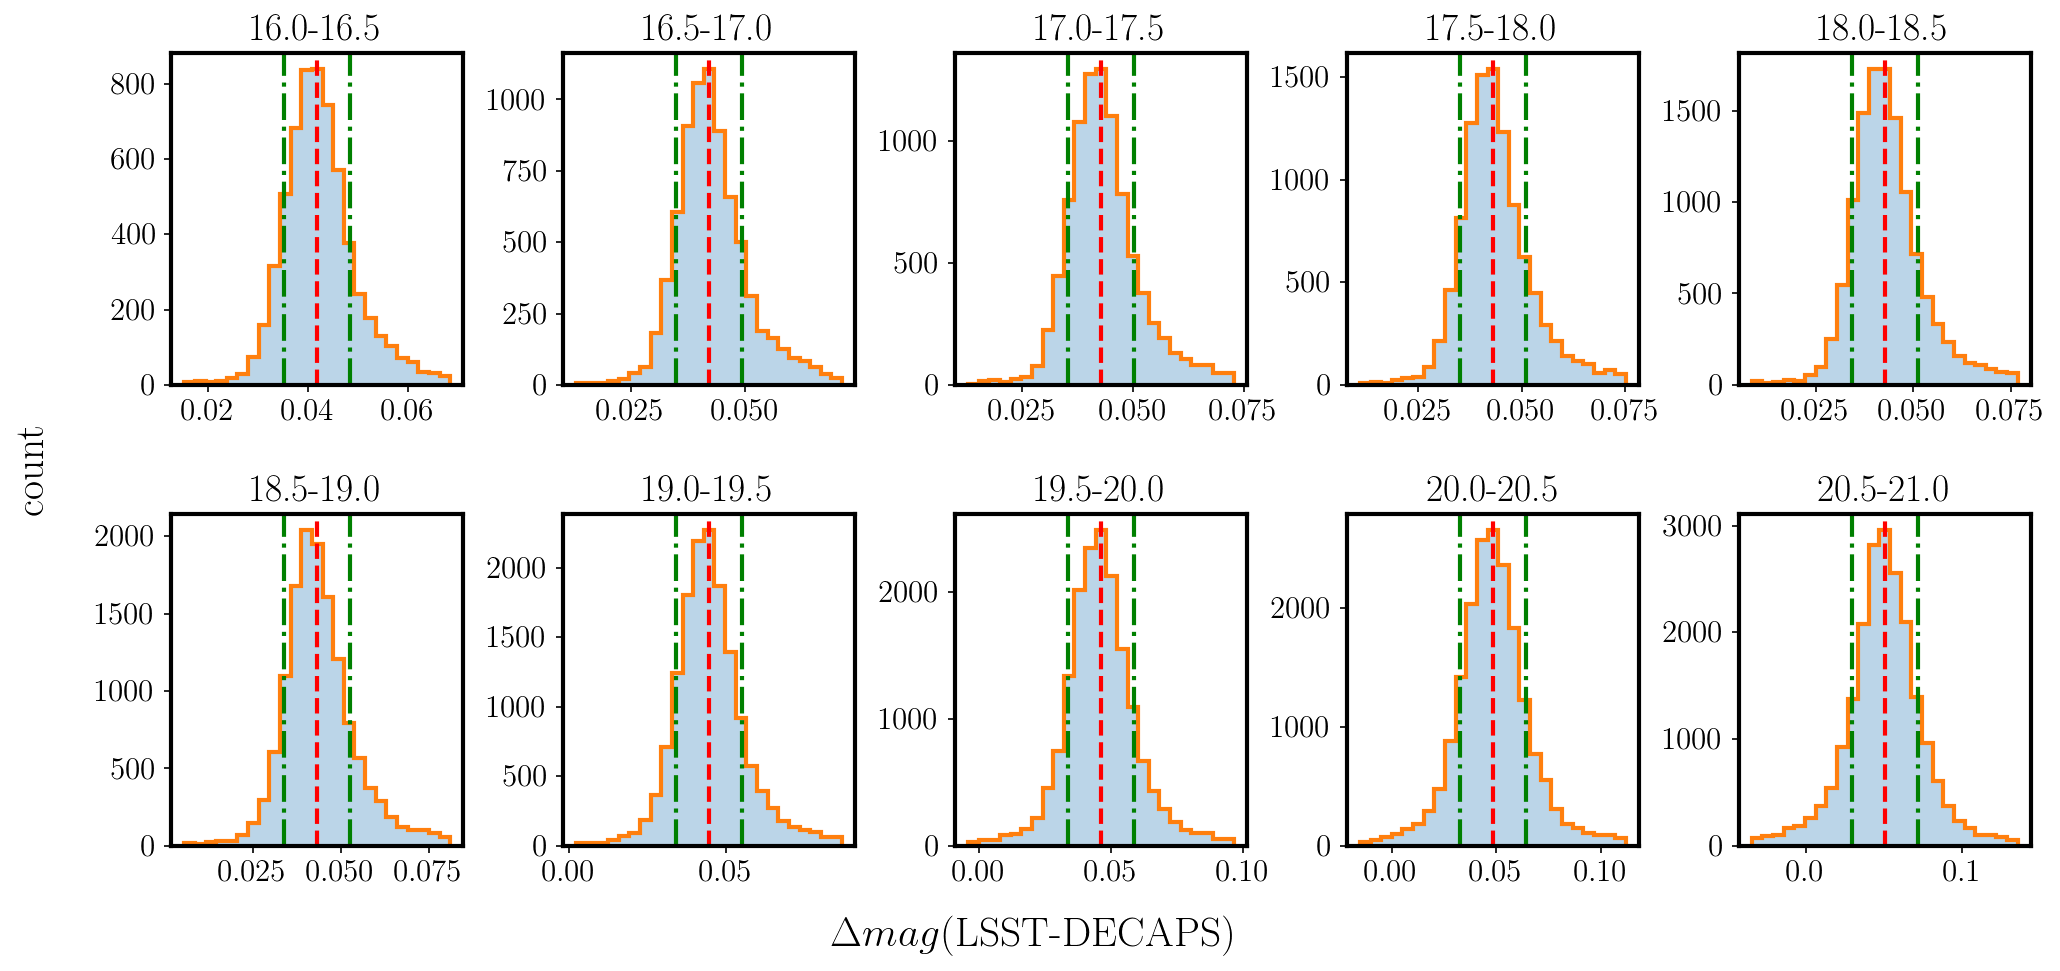
\includegraphics[width=1.0\columnwidth]{figs/rms_decaps_lsst_611970hist_panel.png}
%\vskip -0.15in
\caption{Cross-section of Fig.~\ref{fig:dmag_spread}, showing the histogram of magnitude difference per DECAPS magnitude bin, plotting the median as vertical line, with each histogram limited between $\pm 4 \sigma_{G}$. }
\label{fig:dmag_hist}
\end{figure} 


\begin{figure}
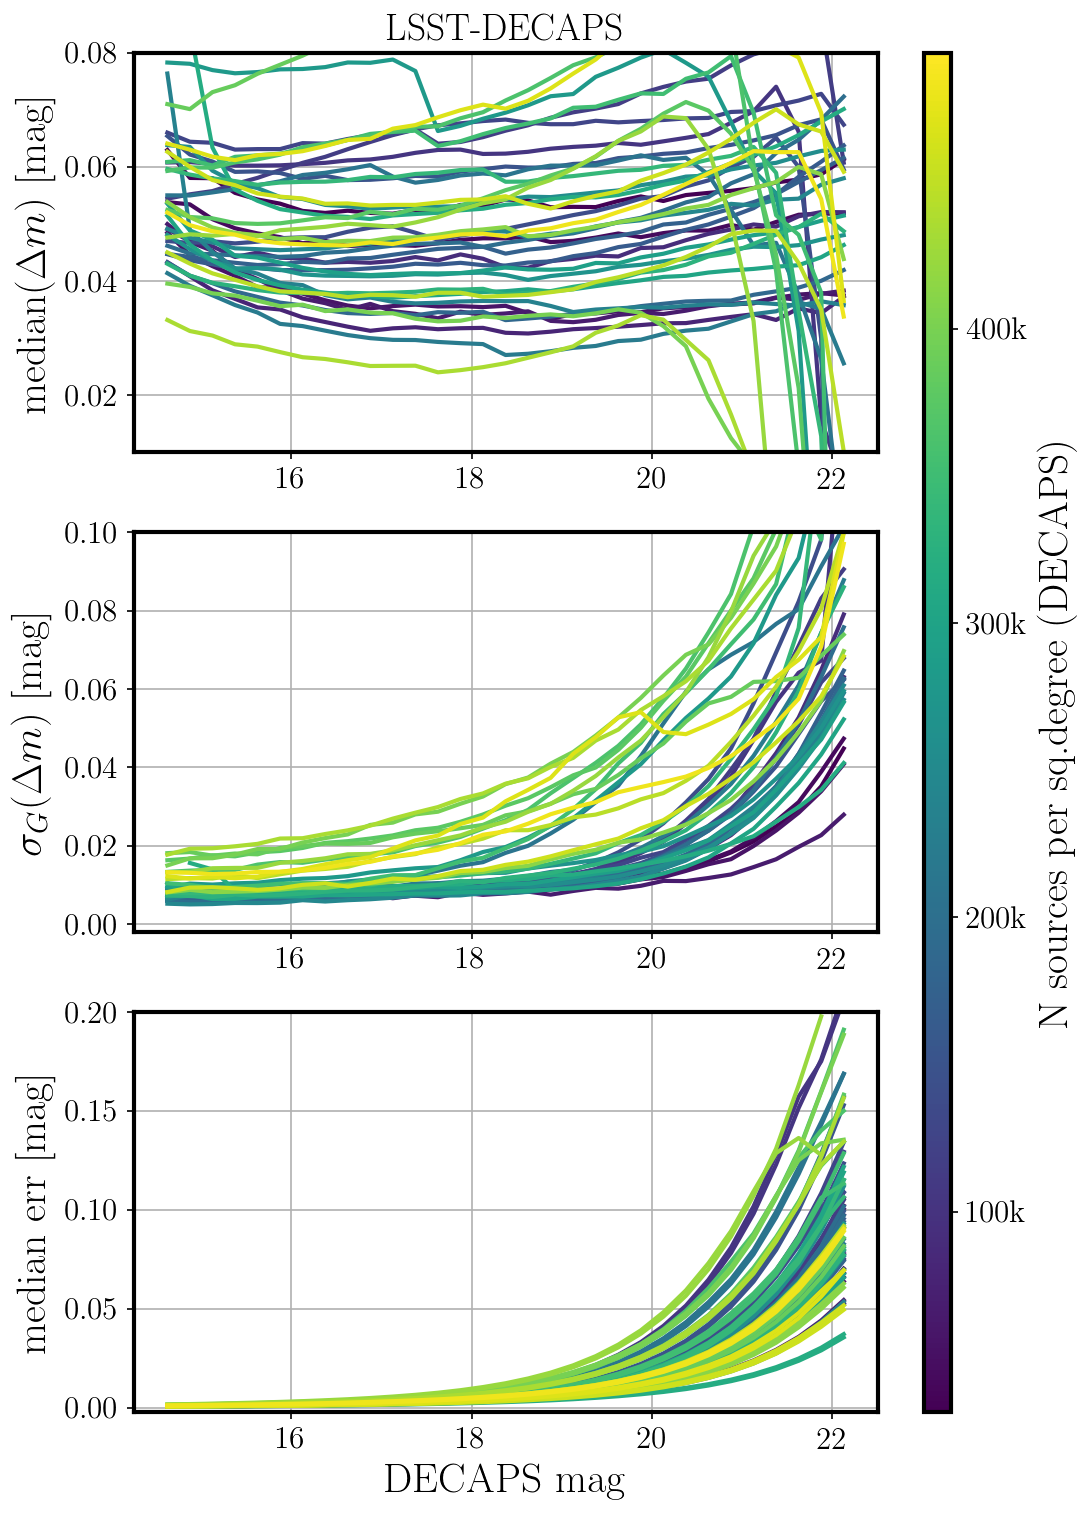
\includegraphics[width=1.0\columnwidth]{figs/decaps_lsst_rms_plot.png}
%\vskip -0.15in
\caption{Median, $\sigma_{G}$, and root-mean-square calculated for fields of different stellar density. Fields at different locations but similar source densities have the same color, but different markers. }
\label{fig:dmag_spread}
\end{figure} 


\section{Conclusion and future work}



\subsection{LSST Processing of StarFast Simulated Sky}
An independent way to further test the performance of the LSST Science Pipelines is to use the simulated sky images, where the true position and  brightness of each source is known. This would put the measure of source detection completeness, photometric and astrometric precision on an absolute scale. We already tested a StarFast image simulator\footnote{\url{https://dmtn-012.lsst.io}}, and confirmed that it can successfully simulate a region of the sky seeded with known stellar population.  

\subsection{Other LSST-DECAPS tests: w-color }



\appendix
\section{Appendix A: TRILEGAL and DAOPhot}
\label{sec:appendixA}


\subsection{DAOStarFinder source detection}
Per each density regime, we performed source extraction with DAOStarFinder\footnote{\url{http://photutils.readthedocs.io/en/stable/photutils/detection.html}}.  This tool uses a classic DAOFIND algorithm~\citep{stetson1987}, and  we used it to verify the plausibility of the MAF source densities using real data.  We performed a straightforward DAOPhot source extraction setting  the detection threshold at $5 \sigma$ level, setting the detection threshold at $5\sigma$. 

\subsection{TRILEGAL queries}
For the same regions of the sky we also  obtained TRILEGAL\footnote{\url{http://stev.oapd.inaf.it/cgi-bin/trilegal}} simulation results, keeping  r < 24.5  sources, with all other run settings as default.  


\subsection{Comparison of MAF, DAOStarFinder, and TRILEGAL counts}
We used the number of sources per TRILEGAL output file, and scaled it to the degree level to compare with MAF and DAO.  The results are shown in Tables ~\ref{tab:one_perc}, ~\ref{tab:five_perc} ,~\ref{tab:twenty_perc} ,~\ref{tab:fifty_perc} for 1\%,5\%,20\% and 50 \% density levels. 


% 1 percent 

\begin{table}
\begin{tabular}{cccccc}
archive & l & b & TRILEGAL & MAF & DAO \\
c4d\_140624\_080728\_ooi\_r & 13.70 & -4.43 & 7,960,511 & 2,650,680 & 498,760 \\
c4d\_170428\_094150\_ooi\_g & 356.86 & -3.90 & 39,852,793 & 4,587,804 & 375,980 \\
c4d\_170501\_055757\_ooi\_g & 356.26 & 5.05 & 16,352,821 & 2,659,968 & 285,630 \\
c4d\_170504\_084722\_ooi\_g & 4.26 & 5.15 & 15,586,874 & 2,833,740 & 561,795 \\
\end{tabular}
\caption{Source density comparison for 1\% density level : TRILEGAL, DAO and MAF columns contain stellar counts from TRILEGAL simulation , DAOStarFinder based on DECam data, and MAF simulation, respectively. All counts are in stars per square degree. }
\label{tab:one_perc}
\end{table}
 

% images of 1 and 5 percent regions 
\begin{figure}
\begin{minipage}[t]{0.5\linewidth}
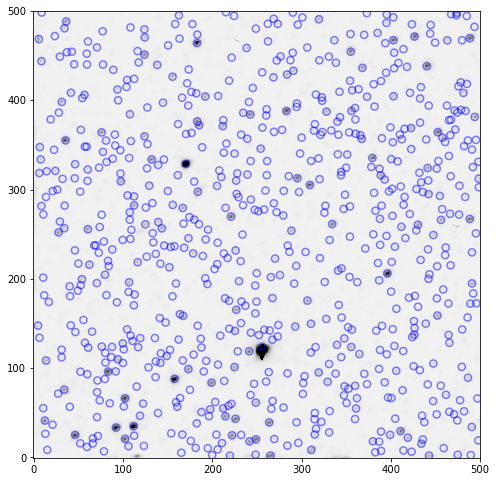
\includegraphics[width=\linewidth]{figs/c4d_170504_084722_ooi_g_v1_1_sub_500px.png}
\caption{500x500 pixels (135x135 arcseconds)  subregion of DECam field c4d\_170504\_084722\_ooi\_g,
a top 1\% density region. With DAOPhot threshold set at 5 $\sigma$,  we detected 722 sources in this postage stamp miniature, corresponding to the area of 0.001406 sq degrees, which translates to 513,422 sources per square degree. At the same coordinates, MAF density is 2,833,740 sources per square degree, and TRILEGAL density is 15,586,874 sources per square degree. }
\label{fig:decam_1_perc_miniature}
\end{minipage}
\hfill
\begin{minipage}[t]{0.5\linewidth}
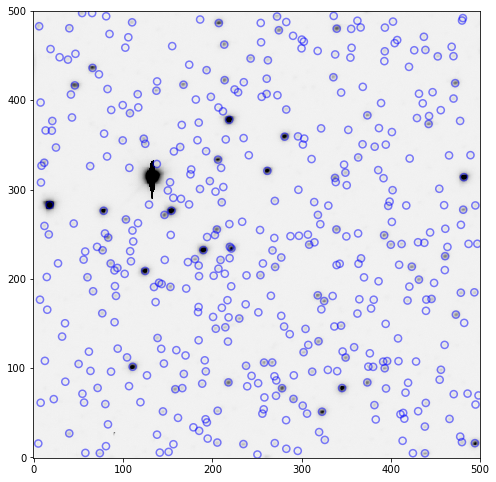
\includegraphics[width=\linewidth]{figs/c4d_170429_035748_ooi_g_v1_1_sub_500px.png}
\caption{500x500 pixels (135x135 arcseconds) subregion of DECam field c4d\_170429\_035748\_ooi\_g,  with 436  detected sources, in the 5 \% density region. The same DAOPhot settings as Fig.~\ref{fig:decam_1_perc_miniature}. That many sources in an area of 0.001406 sq degrees,  translates to 310,044 sources per square degree. At the same coordinates, MAF density is 807,156 sources per square degree, and TRILEGAL density is 1,870,414 sources per square degree. }
\label{fig:decam_5_perc_miniature}
\end{minipage}%
\end{figure}


% 5 percent
\begin{table}
\begin{tabular}{cccccc}
archive & l & b & TRILEGAL & MAF & DAO \\
c4d\_160316\_065235\_ooi\_g & 301.42 & 3.40 & 1,606,135 & 591,336 & 179,277 \\
c4d\_160825\_231905\_ooi\_g & 314.05 & 3.08 & 2,564,964 & 589,572 & 127,088 \\
c4d\_170429\_035748\_ooi\_g & 310.43 & -4.02 & 1,870,414 & 807,156 & 327,483 \\
tu1677011 & 4.48 & 8.70 & 2,530,163 & 810,144 & 509,093 \\
\end{tabular}
\caption{Source density comparison for 5\% density level, all columns and units as in Table ~\ref{tab:one_perc}}
\label{tab:five_perc}
\end{table}



% 21 percent 
\begin{table}
\begin{tabular}{cccccc}
archive & l & b & TRILEGAL & MAF & DAO \\
c4d\_170122\_055542\_ooi\_g & 242.43 & 3.77 & 341,343 & 116,856 & 66,282 \\
tu1661798 & 351.66 & 20.42 & 183,778 & 118,188 & 44,216 \\
tu1668579 & 217.04 & 1.21 & 379,319 & 111,096 & 54,004 \\
tu2187073 & 312.84 & 14.64 & 184,583 & 107,784 & 60,678 \\
\end{tabular}
\caption{Source density comparison for 20\% density level, all columns and units as in Table ~\ref{tab:one_perc}}
\label{tab:twenty_perc}
\end{table}

% images of 21 and 51 percent regions 

\begin{figure}
\begin{minipage}[t]{0.5\linewidth}
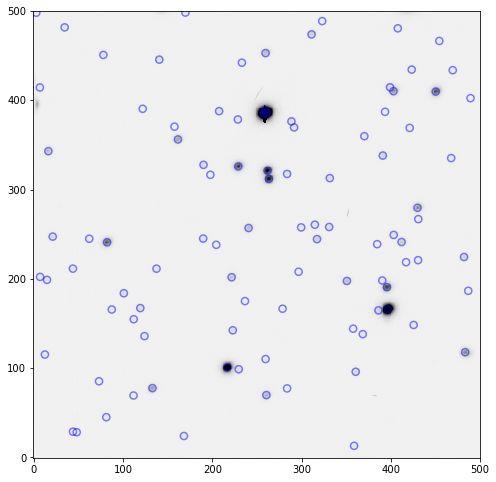
\includegraphics[width=\linewidth]{figs/c4d_170122_055542_ooi_g_v1_1_sub_500px.png}
\caption{500x500 pixels (135x135 arcseconds) subregion of DECam field c4d\_170122\_055542\_ooi\_g,  with 98  detected sources, in the  20 \% density region. The same DAOPhot settings as Fig.~\ref{fig:decam_1_perc_miniature}. That many sources in an area of 0.001406 sq degrees,  translates to 69,688 sources per square degree. At the same coordinates,  MAF density is  116,856 sources per square degree, and TRILEGAL density is 341,343 sources per square degree. }
\label{fig:decam_20_perc_miniature}
\end{minipage}
\hfill
\begin{minipage}[t]{0.5\linewidth}
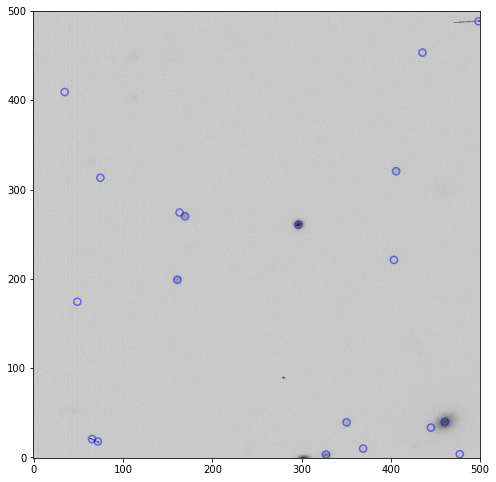
\includegraphics[width=\linewidth]{figs/c4d_160607_025052_ooi_g_v1_1_sub_500px.png}
\caption{500x500 pixels (135x135 arcseconds) subregion of DECam field c4d\_160607\_025052\_ooi\_g,  with 19  detected sources, in the  50 \% density region. The same DAOPhot settings as Fig.~\ref{fig:decam_1_perc_miniature}. That many sources in an area of 0.001406 sq degrees,  translates to 13,511 sources per square degree. At the same coordinates, MAF density is  20,052 per square degree, and TRILEGAL density is 29,607 sources per square degree.}
\label{fig:decam_20_perc_miniature}
\end{minipage}%
\end{figure}


% 51 percent  
\begin{table}
\begin{tabular}{cccccc}
archive & l & b & TRILEGAL & MAF & DAO \\
c4d\_150615\_005257\_ooi\_g & 344.39 & 41.67 & 27,633 & 21,024 & 12,904 \\
c4d\_160607\_025052\_ooi\_g & 2.92 & 41.68 & 29,607 & 20,052 & 13,371 \\
c4d\_160825\_034122\_ooi\_g & 345.83 & 1.28 & 18,364,268 & 20,268 & 91,177 \\
tu2046406.fits.fz & 220.89 & -16.08 & 41,832 & 19,944 & 35,974 \\
\end{tabular}
\caption{Source density comparison for 50\% density level, all columns and units as in Table ~\ref{tab:one_perc}}
\label{tab:fifty_perc}
\end{table}


%%%%%%%%%%%%%%%%%%%%%%%%%%%%%%%%%%%%%%%%%%%%%%%%%%
%%%%%%%%%%%%%%%%%%%% REFERENCES %%%%%%%%%%%%%%%%%%
%%%%%%%%%%%%%%%%%%%%%%%%%%%%%%%%%%%%%%%%%%%%%%%%%%

\bibliographystyle{apj}
\bibliography{references}
\end{document}